\documentclass[11pt]{article}

%%%%%%%%%%%%%%%%%%%%%%%%%%%%%%%%%%%%%%%%%%%%%%%%%%%%%%%%%%%%%%%%%%%%%%%%%%%%%%%%
% packages
%%%%%%%%%%%%%%%%%%%%%%%%%%%%%%%%%%%%%%%%%%%%%%%%%%%%%%%%%%%%%%%%%%%%%%%%%%%%%%%%

\usepackage{coling2020}
\usepackage{times}
\usepackage{url}
\usepackage{amsmath,amsfonts}
\usepackage{latexsym}
\usepackage{hyperref}
\hypersetup{
  colorlinks   = true, %Colours links instead of ugly boxes
  urlcolor     = blue, %Colour for external hyperlinks
  linkcolor    = blue, %Colour of internal links
  citecolor    = blue  %Colour of citations
}
\usepackage{CJKutf8}
\usepackage{subfig}
\usepackage[sort&compress,round,comma,authoryear]{natbib}
\usepackage{booktabs}
\usepackage{graphicx}
\usepackage[inline]{enumitem}

\usepackage{graphicx}
\usepackage{grffile}

\usepackage{csquotes}
\renewcommand{\mkbegdispquote}[2]{\itshape}

%%%%%%%%%%%%%%%%%%%%%%%%%%%%%%%%%%%%%%%%%%%%%%%%%%%%%%%%%%%%%%%%%%%%%%%%%%%%%%%%
% latex functions
%%%%%%%%%%%%%%%%%%%%%%%%%%%%%%%%%%%%%%%%%%%%%%%%%%%%%%%%%%%%%%%%%%%%%%%%%%%%%%%%

\newcommand{\ltwo}[1]{\lVert{#1}\rVert}
\newcommand{\indicator}[1]{\mathbbm{1}\!\left[{#1}\right]}
\newcommand{\R}{\mathbb R}
\newcommand{\TEXT}{\texttt{text}}

\newcommand{\defn}[1]{\emph{{#1}}}
%\newcommand{\fixme}[1]{{\color{red} \textbf{FIXME:} {\textit {#1}}}}
\newcommand{\fixme}[1]{}
\newcommand{\XXX}{{\color{red}\textbf{XXX}}~}
\newcommand{\bertmoji}{\texttt{BERTmoticon}}
\newcommand{\bertmojill}{\texttt{BERTmoticon-LL}}
%\newcommand{\bert}{\texttt{BERT-multilingual}}
\newcommand{\bert}{\text{multilingual BERT}}
\newcommand{\spacy}{\texttt{spaCy}}


\newcommand{\emoji}[1]{\includegraphics[height=\fontcharht\font`\B]{./images/#1}}
%\newcommand{\emoji}[1]{\includegraphics[height=0.8em,trim=0 0.3em 0 -0.3em]{images/{#1}}}
%\newcommand{\emoji}[1]{${}_{\includegraphics[height=\fontcharht\font`\B]{images/{#1}}}$}

\DeclareMathOperator*{\argmax}{arg\,max}
\DeclareMathOperator*{\argmin}{arg\,min}
\DeclareMathOperator{\acc}{acc}
\DeclareMathOperator{\none}{\texttt{None}}
%\DeclareMathOperator{\model}{\texttt{BERTMultilingualEmoticon}}
\DeclareMathOperator{\emoticon}{\texttt{TwitterEmoticon}}
\DeclareMathOperator{\emoticonTrain}{\texttt{TwitterEmoticon\_train}}
\DeclareMathOperator{\emoticonValid}{\texttt{TwitterEmoticon\_valid}}
\DeclareMathOperator{\emoticonTest}{\texttt{TwitterEmoticon\_test}}
\DeclareMathOperator{\corona}{\texttt{TwitterCOVID}}

%%%%%%%%%%%%%%%%%%%%%%%%%%%%%%%%%%%%%%%%%%%%%%%%%%%%%%%%%%%%%%%%%%%%%%%%%%%%%%%%
% paper configuration
%%%%%%%%%%%%%%%%%%%%%%%%%%%%%%%%%%%%%%%%%%%%%%%%%%%%%%%%%%%%%%%%%%%%%%%%%%%%%%%%

\setlength\titlebox{5cm}
\colingfinalcopy % Uncomment this line for the final submission

% You can expand the titlebox if you need extra space
% to show all the authors. Please do not make the titlebox
% smaller than 5cm (the original size); we will check this
% in the camera-ready version and ask you to change it back.

\title{Multilingual Emoticon Prediction of Tweets about COVID-19 \emoji{mask_photo.png} }

\author{Stefanos Stoikos \\
  Pomona College\\

  {\tt st.stoikos@gmail.com} \\\And
  Mike Izbicki \\
  Claremont Mckenna College\\
  {\tt mike@izbicki.me} \\}

\date{}

%%%%%%%%%%%%%%%%%%%%%%%%%%%%%%%%%%%%%%%%%%%%%%%%%%%%%%%%%%%%%%%%%%%%%%%%%%%%%%%%
% document text
%%%%%%%%%%%%%%%%%%%%%%%%%%%%%%%%%%%%%%%%%%%%%%%%%%%%%%%%%%%%%%%%%%%%%%%%%%%%%%%%

\begin{document}
\maketitle
\begin{abstract}
    %There are no multi-lingual emoji prediction models. This makes it hard to investigate
    %how different languages use emojis. We present $\bertmoji$, a multi-lingual model 
    %that fine tunes the \texttt{BERTMultilingual} to the emoji prediction task.
    Emojis are a widely used tool for encoding emotional content in informal messages such as tweets,
    and predicting which emoji corresponds to a piece of text can be used as a proxy for measuring the emotional content in the text.
    This paper presents the first model for predicting emojis in highly multilingual text.
    Our $\bertmoji$ model is a fine-tuned version of the $\bert$ model \citep{devlin2018bert},
    and it can predict emojis for text, written in 102 different languages.
    We trained our $\bertmoji$ model on 54.2 million geolocated tweets sent in the first 6 months of 2020,
    and we apply the model to a case study analyzing the emotional reaction of Twitter users to news about the coronavirus.
    Example findings include a spike in sadness when the World Health Organization (WHO) declared that coronavirus was a global pandemic,
    and a spike in anger and disgust when the number of COVID-19 related deaths in the United States surpassed one hundred thousand.
    We provide an easy-to-use and open source python library for predicting emojis with $\bertmoji$ so that the model can easily be applied to other data mining tasks.
\end{abstract}

%
% The following footnote without marker is needed for the camera-ready
% version of the paper.
% Comment out the instructions (first text) and uncomment the 8 lines
% under "final paper" for your variant of English.
% 
\blfootnote{
    %
    % for review submission
    %
    \hspace{-0.65cm}  % space normally used by the marker
    %Place licence statement here for the camera-ready version. 
    %
    % % final paper: en-uk version 
    %
    % \hspace{-0.65cm}  % space normally used by the marker
    % This work is licensed under a Creative Commons 
    % Attribution 4.0 International Licence.
    % Licence details:
    % \url{http://creativecommons.org/licenses/by/4.0/}.
    \hspace{-0.65cm}  % space normally used by the marker
    This work is licensed under a Creative Commons 
    Attribution 4.0 International License.
    License details:
    \url{http://creativecommons.org/licenses/by/4.0/}.
}





\section{Introduction}
\label{sec:intro}

The COVID-19 pandemic has caused intense emotional reactions on social media.
Some tweets are sad:
\begin{displayquote}
    This Corona stuff is no joke. Watching people get laid off at work today really made me open my eyes. Wish it was all over. 
    \emoji{loudly-crying-face_1f62d} 
    \emoji{anguished-face_1f627}
    \emoji{folded-hands_1f64f}
\end{displayquote}
And other tweets are angry:
\begin{displayquote}
    I saw that bottles of Purell were selling for \$149! Go away price gougers and go away coronavirus! 
    \emoji{angry-face_1f620}
    \emoji{angry-face_1f620}
    \emoji{angry-face_1f620}
    \emoji{angry-face_1f620}
    \emoji{angry-face_1f620}
    \emoji{angry-face_1f620}
    %\emoji{pouting-face_1f621}
    %\emoji{pouting-face_1f621}
\end{displayquote}
What both of these tweets have in common is that their emotional content is captured by emojis present in the tweet's text.
Emojis are often used in informal tweets sent between friends \citep{marcel2016emoji},
but most tweets do not contain emojis.
For example, the following tweet by the BBC (a major British newspaper) is clearly meant to help us find joy amidst the stress of COVID-19:
\begin{displayquote}
    Father dresses as Transformers character Bumblebee to surprise his son on his first day back at school after lockdown.
\end{displayquote}
But there are no emojis in the text to indicate that the tweet is joyful.
One possible emoji for this tweet would be the ``grinning face'' (\emoji{grinning-face_1f600}),
but more subtle emojis like ``grinning face with tongue'' (\emoji{face-with-tongue_1f61b}) or ``grinning face with smiling eyes'' (\emoji{grinning-face-with-smiling-eyes_1f604}) would also be appropriate and convey slightly different emotions.
%Based on analysis of our $\corona$ dataset (discussed in detail below),
%only \XXX percent of tweets about the coronavirus contain emojis.
The goal of this paper is to automatically annotate these emoji-less tweets with appropriate emojis in order to better understand the emotional content in online discussions of COVID-19.
%Annotating tweets with appropriate emojis is a difficult task that requires understanding subtle textual cues.
%This is a difficult task because many tweets can reasonably be labeled with different emojis,
%and the textual cues indicating emotional content are subtle.

\begin{figure}
    \centering
    %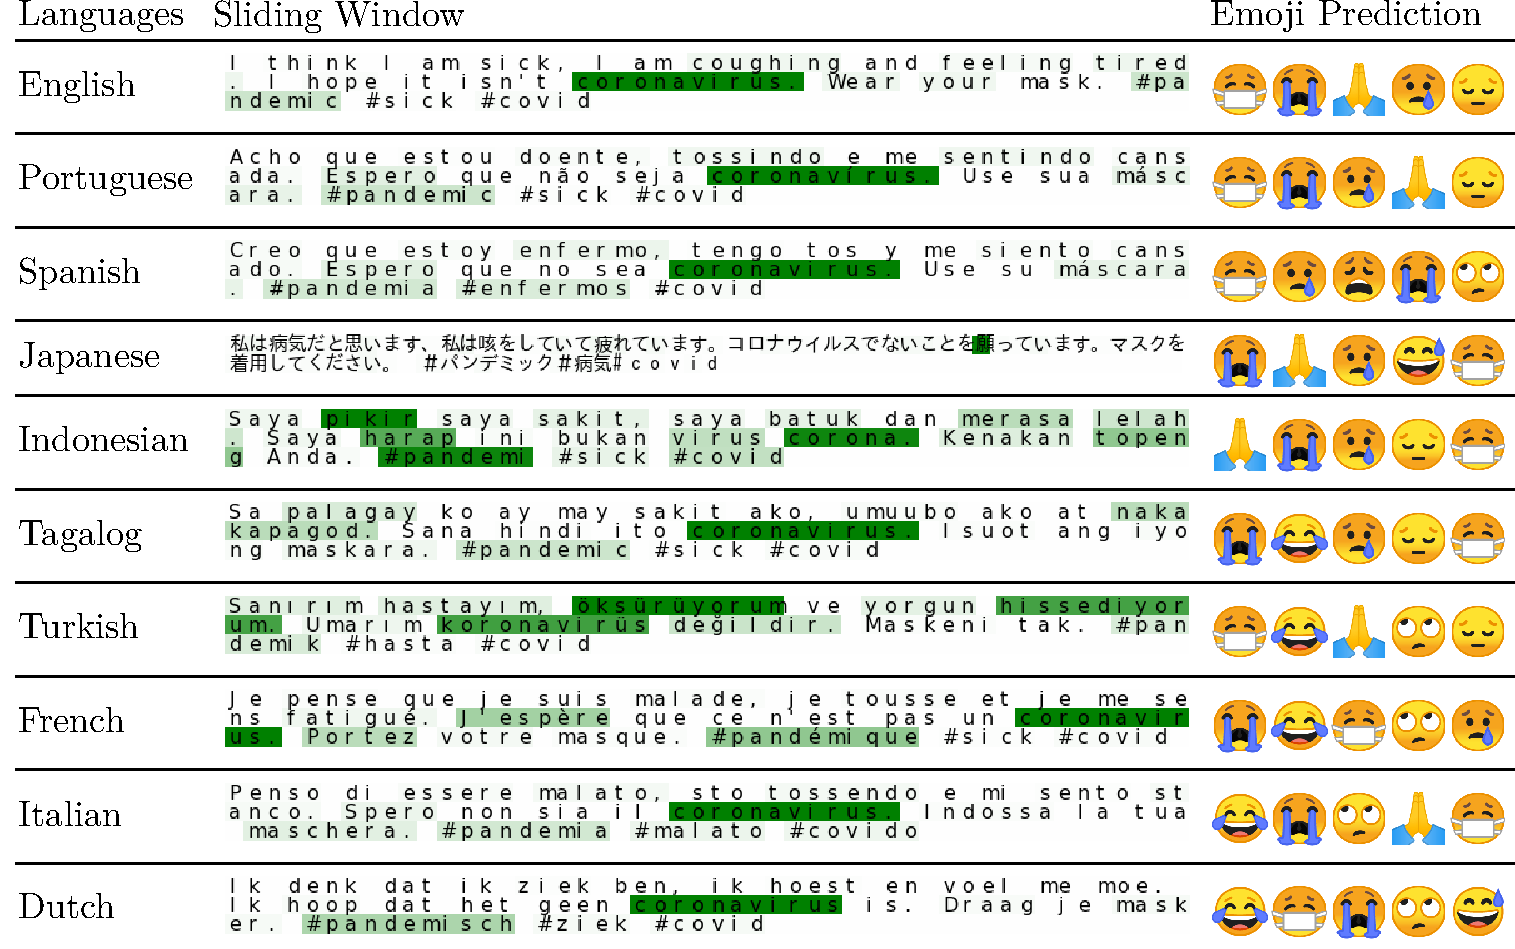
\includegraphics[width=\textwidth]{images/languages_slide_fix.pdf}
    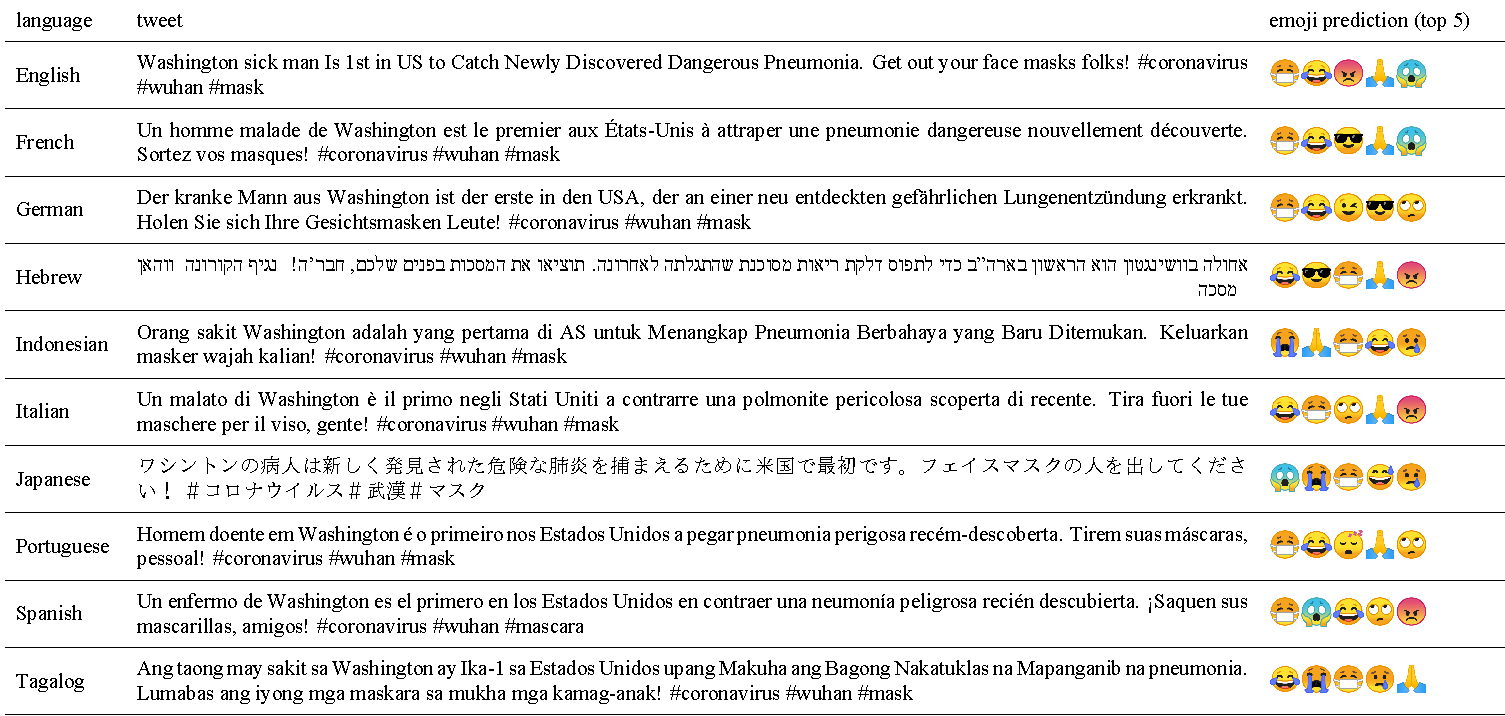
\includegraphics[height=3in]{images/translations_fixed.pdf}
    \caption{
        $\bertmoji$ predicts good emojis in a wide variety of languages.
        All non-English text above was translated from the English using Google Translate.
        \fixme{Hebrew text should be right aligned and written right to left.  It looks like each individual word is right to left, but the words are arranged left to right.}
     }
    \label{fig:prediction_top10_langs}
\end{figure}


%Emojis are well known to encode the emotional content of tweets \citep{sari2014user,kralj2015sentiment,eisner2016emoji2vec,wood2016emoji,felbo2017using,shoeb2019emotag}.
%Emoji prediction is therefore a more attractive task than direct emotion prediction because of the difficulty in obtaining quality emotion labels.
%\citet{mozetivc2016multilingual} show that human annotators are incredibly difficult to coordinate in multilingual sentiment evaluation tasks.
%And therefore several works have tackled the problem of predicting emojis from a tweet's text as a proxy for predicting emotion \citep{barbieri2017emojis,felbo2017using,Zhang2019}.
Prior work on predicting emojis from the text of a tweet \citep{barbieri2017emojis,felbo2017using,Zhang2019} has focused only on English language tweets.
Models submitted for the SemEval 2018 Task 2 \citep{barbieri2018semeval} are the most multilingual emoji prediction models currently published,
but this task considered only English and Spanish tweets.
Because COVID-19 is a worldwide phenomenon, however, to understand emotional responses to COVID-19, we must be able to predict emojis in all languages used on Twitter.
We therefore introduce the first highly multilingual model for emoji prediction, which we call $\bertmoji$.
Our model is based on fine-tuning the multilingual BERT model \citep{devlin2018bert},
which was trained on a dataset of 102 distinct languages.
Figure \ref{fig:prediction_top10_langs} shows the output of our model on a tweet translated into ten different languages.
%Emojis are rendered differently across different platforms, leading to translation issues \citep{miller2018see}

%Following the work of \citet{fixme1,fixme2,fixme3}, we use emojis as distant labels for emotions.
%Hand classifying text by emotions is an expensive and error prone process,
%and the largest existing datasets for this task contain only about 10,000 tweets focusing on the limited domains of video games \citep{fixme} or stock performance \citep{fixme}.

%In the times that we are facing, exploring the public's sentiment offers useful insight into how people react to situations of stress, anxiety and uncertainty. A perfect source to explore this is through Twitter's API.\cite{subasish2020} draws from tweets related to Covid19 and India and by using public available sentiment analysis tools explores the public's sentiment on a two sentiment basis (negative and positive). 
A large body of work has emerged analyzing tweets about COVID-19.
One prominent line of research attempts to identify how misinformation about the disease spreads online \citep{kouzy2020coronavirus,sharma2020coronavirus,yang2020prevalence,elhadad2020covid,prabhakar2020informational}.
An important subcategory of this research investigates the spread of racist \citep{budhwani2020creating,schild2020go} and ageist \citep{jimenez2020coronavirus} misinformation.
Other research more similar to our own investigates the sentiment of tweets about the coronavirus.
Some of this research focuses on specific locations such as Belgium \citep{kurten2020coronavirus}, Paris \citep{saire2020study}, Poland \citep{jarynowski2020perception} or India \citep{subasish2020}.
Other research studies English-language tweets \citep{rajput2020word,yin2020detecting} over wider geographic areas.
Our research stands out from this prior work in two important ways.
First, we do not consider a subset of tweets about COVID-19,
we consider all tweets, written in all languages, sent from anywhere in the world.
This is a significantly more challenging technical problem than previous research addressed,
but it is also much more useful.
Second, we are the first paper to consider the more general emoji prediction problem rather than the sentiment prediction problem.
In sentiment prediction,
the goal is to assign a positive or negative sentiment to each tweet,
and for the coronavirus topic it can be difficult to decidedly assign one sentiment. Tweets about COVID-19 can express negative sentiments because the disease has killed millions of people and forced us to make drastic changes to our lifestyles but also can contain funny, uplifting content exhibiting a positive sentiment such as:

\begin{displayquote}
    Happy \#NationalCatDay from my beautiful adopted pandemic pet!   
\end{displayquote}

In the emoji prediction task, we are able to get a more fine-tuned emotional understanding of tweets. For example, we can answer questions like: is the tweet sad? angry? joyful?

%college students respond differently \citep{duong2020ivory}
%map travel patterns using geotagged tweets \citep{feng2020working}

Our contributions are as follows.
In Section \ref{sec:bertmoji} we introduce the first dataset for training highly multilingual emoji prediction models, $\emoticon$.
We then use this dataset to train the first highly multilingual emoticon prediction model, $\bertmoji$.
Our model is open source and has an easy to use PyPi package.%
\footnote{
    \url{https://pypi.org/project/bertmoticon/}
}
In Section \ref{sec:casestudy}, we introduce the first highly multilingual dataset of tweets about COVID-19, called $\corona$.
To generate the dataset, we introduce a novel dataset generation method combining the Twitter API, Bing Translate, and the $\spacy$ tokenization library \citep{spacy2}.
We then apply the $\bertmoji$ model to the $\corona$ dataset to map how Twitter users across the world have emotionally responded to a variety of COVID-19 news events.
This is the first highly multilingual emotion analysis of tweets in any language,
and by far the most comprehensive analysis to-date specifically about the COVID-19 pandemic.

%%%%%%%%%%%%%%%%%%%%%%%%%%%%%%%%%%%%%%%%%%%%%%%%%%%%%%%%%%%%%%%%%%%%%%%%%%%%%%%%

\section{The $\bertmoji$ Model}
\label{sec:bertmoji}

In this section, we first describe the emoticons we are trying to predict and present the $\emoticon$ dataset that the $\bertmoji$ model was trained on.
Then we describe our training procedure and model evaluation results.
We take particular care to ensure that the $\emoticon$ dataset is sampled from a similar distribution to the $\corona$ dataset analyzed in Section \ref{sec:casestudy} below in order to ensure that the $\bertmoji$ model will transfer well to this unlabeled dataset.
%The purpose of the $\emoticon$ dataset is to develop the emotion classifier which we will later use in our case study of coronavirus-specific tweets.
%The $\emoticon$ dataset is large, with \XXX million tweets in at least 66 languages sampled from the same distribution as our coronavirus tweets.
%Therefore, we can expect a classifier trained on the $\emoticon$ dataset to transfer well to the $\corona$ dataset.

%%%%%%%%%%%%%%%%%%%%%%%%%%%%%%%%%%%%%%%%

\subsection{The Target Emoticons}

\begin{figure}
    \centering
    \subfloat{{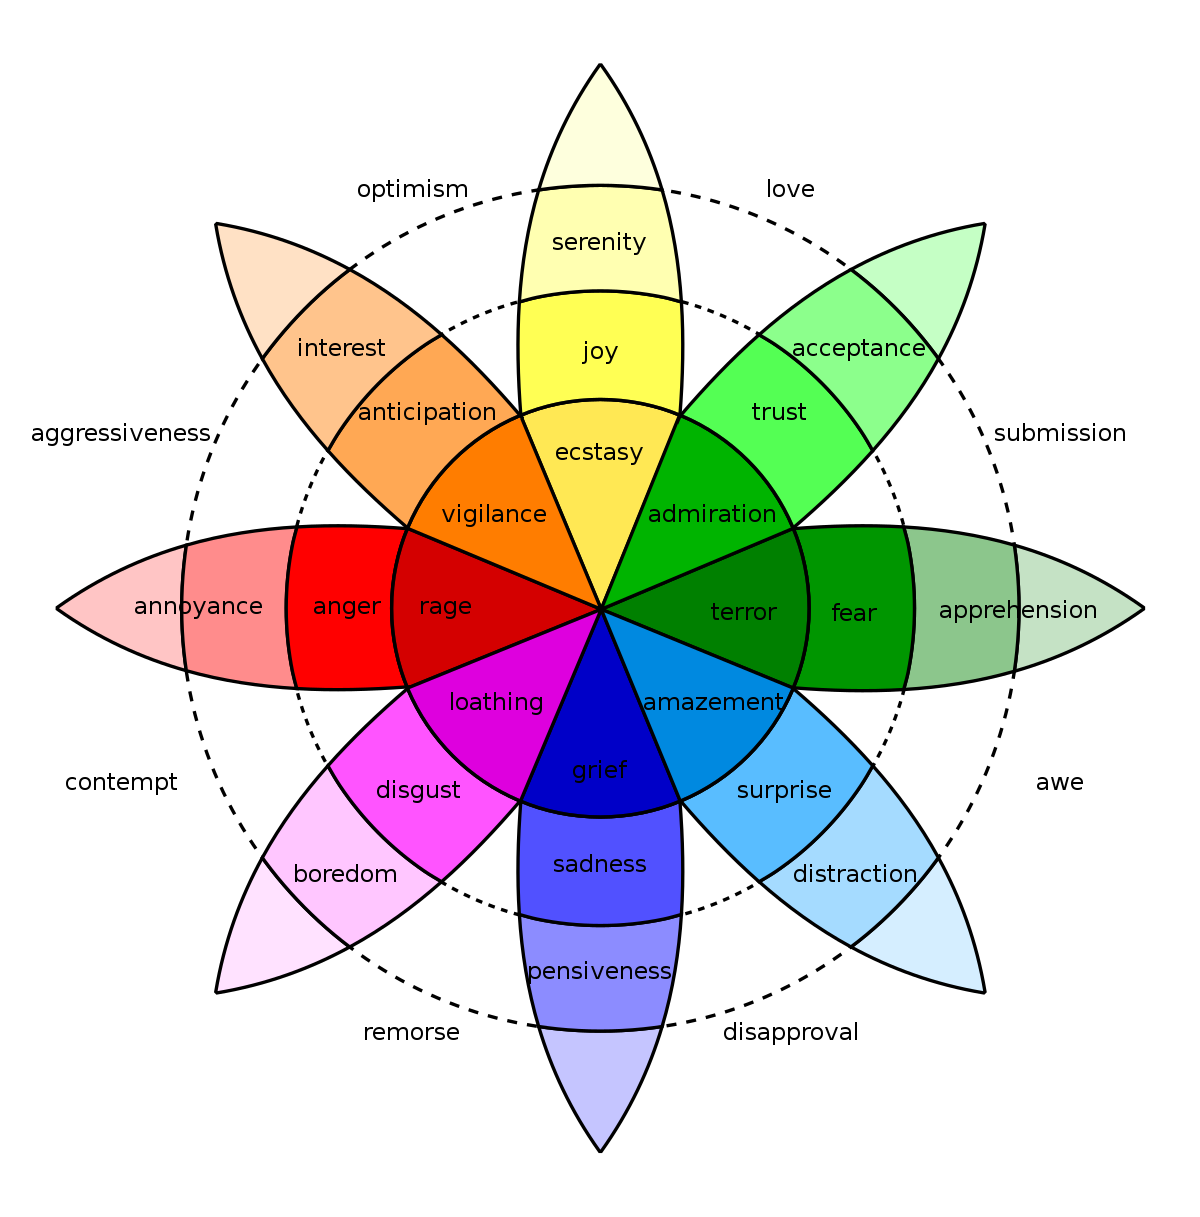
\includegraphics[scale=0.125]{images/Plutchik-wheel.png}}}%
    \label{fig:plu_wheel}
    \subfloat{{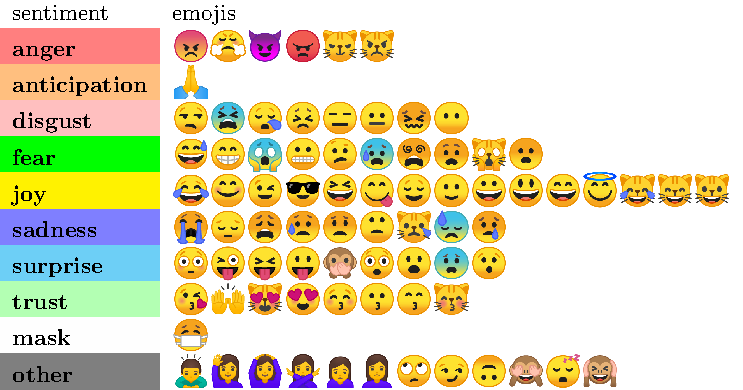
\includegraphics[scale= 0.78]{images/categories_fixed.pdf}}}%
    \caption{
        (\emph{Left}) 
        The Plutchik wheel of emotions.
        %\footnote{\url{https://en.wikipedia.org/wiki/Robert_Plutchik}}
        (\emph{Right}) 
        We have grouped the emoticons into 10 different categories:
        8 emotional categories from the Plutchnik wheel,
        1 category for the ``face with medical mask'' emoticon,
        and 1 category for all other emoticons that represent emotions that are not clearly in the Plutchik wheel.
        %\fixme{
            %You need a label for the emotions column.  You also need to shrink the table vertically so that it's the same exact height as the Plutchik wheel.
        %}
    }
    \label{fig:Mapped_emojis}%
\end{figure}


Emojis were first added to the Unicode standard in 2010,
and the current version of the standard (12.1.0) defines 3304 different emojis \citep{unicode12}.
Prior work on emoji prediction has limited itself to predicting only a subset of the available emojis.
For example, \citet{barbieri2017emojis} consider only the 20 most commonly used emoji,
and DeepMoji \citep{felbo2017using} considers only 64 emoji.
%Both of these models predict emojis only for English text.
There are two primary reasons for only considering a subset of emoji.
First, emoji-usage follows a power law distribution where the top 1\% of most used emoji account for over 99\% of all emoji usage.%
\footnote{
    See \url{http://www.emojitracker.com/} for real-time stats on Twitter emoji usage.
}
There is therefore very little training data for the less popular emojis,
and so we cannot expect a classifier to have high prediction accuracy for these emoji.
Second, many emoji (e.g.\ the Greek Flag emoji \emoji{flag-greece_1f1ec-1f1f7}) do not contain emotional information,
and so the ability to predict these emoji does not help us understand the emotional content of text.

We follow previous work and focus on predicting only a limited set of emoji.
Specifically, we focus on the original 80 emoji defined in the Unicode standard's emoticon code block (code points \texttt{0x1f600} - \texttt{0x1f650}). %\footnote{
    In common usage, the words \defn{emoji} and \defn{emoticon} are interchangeable,
    but in this paper we adopt the Unicode Standard's definitions of these terms.
    By these definitions, an \defn{emoji} is any one of 3304 pictographs that are not part of any written language,
    and an \defn{emoticon} is one of the original 80 emoji defined in the code block specified above.
%}
We limit our analysis to emoticons for three reasons.
First, they are the most commonly used emoji on twitter,
so we can expect to achieve relatively high accuracy.
Second, each emoticon represents an emotion (emoticon is a portmanteau of emotion and icon).
Third, the emoticon block contains the ``face with medical mask'' emoji (\emoji{mask_photo.png}),
which is important for our case study analyzing emotional responses to the coronavirus.

Figure \ref{fig:Mapped_emojis} shows the 80 emoticons and a mapping from these emoticons to the Plutchik wheel of emotions \citep{plutchik1991emotions}.
The Plutchik wheel is a standard psychological model for encoding emotions that has been highly influential in emotion prediction systems \citep[e.g.][]{suttles2013distant,kant2018practical,liu2019dens}.
It has 8 primary emotional categories (anger, anticipation, disgust, fear, joy, sadness, surprise, and trust).
These emotions are arranged spatially so that similar emotions (e.g.\ joy, trust) appear near each other, and dissimilar emotions (e.g.\ joy, sadness) appear opposite each other.
Furthermore, each emotional category is broken down into sub-categories that encode the strength of the emotion (e.g.\ ecstasy is an extreme form of joy, and serenity is a mild form of joy).

There is currently no standard mapping from emoticons onto the Plutchik wheel,
and in Figure \ref{fig:Mapped_emojis} (\emph{right}) we provide a suggested mapping.
To generate this mapping, we manually assigned each emoticon to an emotion based on the description of the emoticon on the website \url{emojipedia.org}.
The mapping is not perfect.
The category joy has many emoticons representing different facets of joy,
but the category anticipation has only a single emoticon.
We emphasize that our $\bertmoji$ model will predict raw emoticons directly,
but we present the mapping onto the Plutchnik wheel emotions to help make the wide array of emoticon emotions more easily understandable.

%We used NVidia's \texttt{sentiment-discovery} library to provide a preliminary sentiment analysis of the $\corona$ dataset,
%and the results are shown in Figure \ref{fig:nvidia-sentiment}.
%The results are not very informative, however, because NVidia's model was trained on a small set of English-language tweets (about 16 thousand) about video games,
%and there is little reason to believe that this domain would transfer well to the coronavirus domain.

%%%%%%%%%%%%%%%%%%%%%%%%%%%%%%%%%%%%%%%%

\subsection{The $\emoticon$ Dataset}

\begin{figure}%
    \centering
    \subfloat{{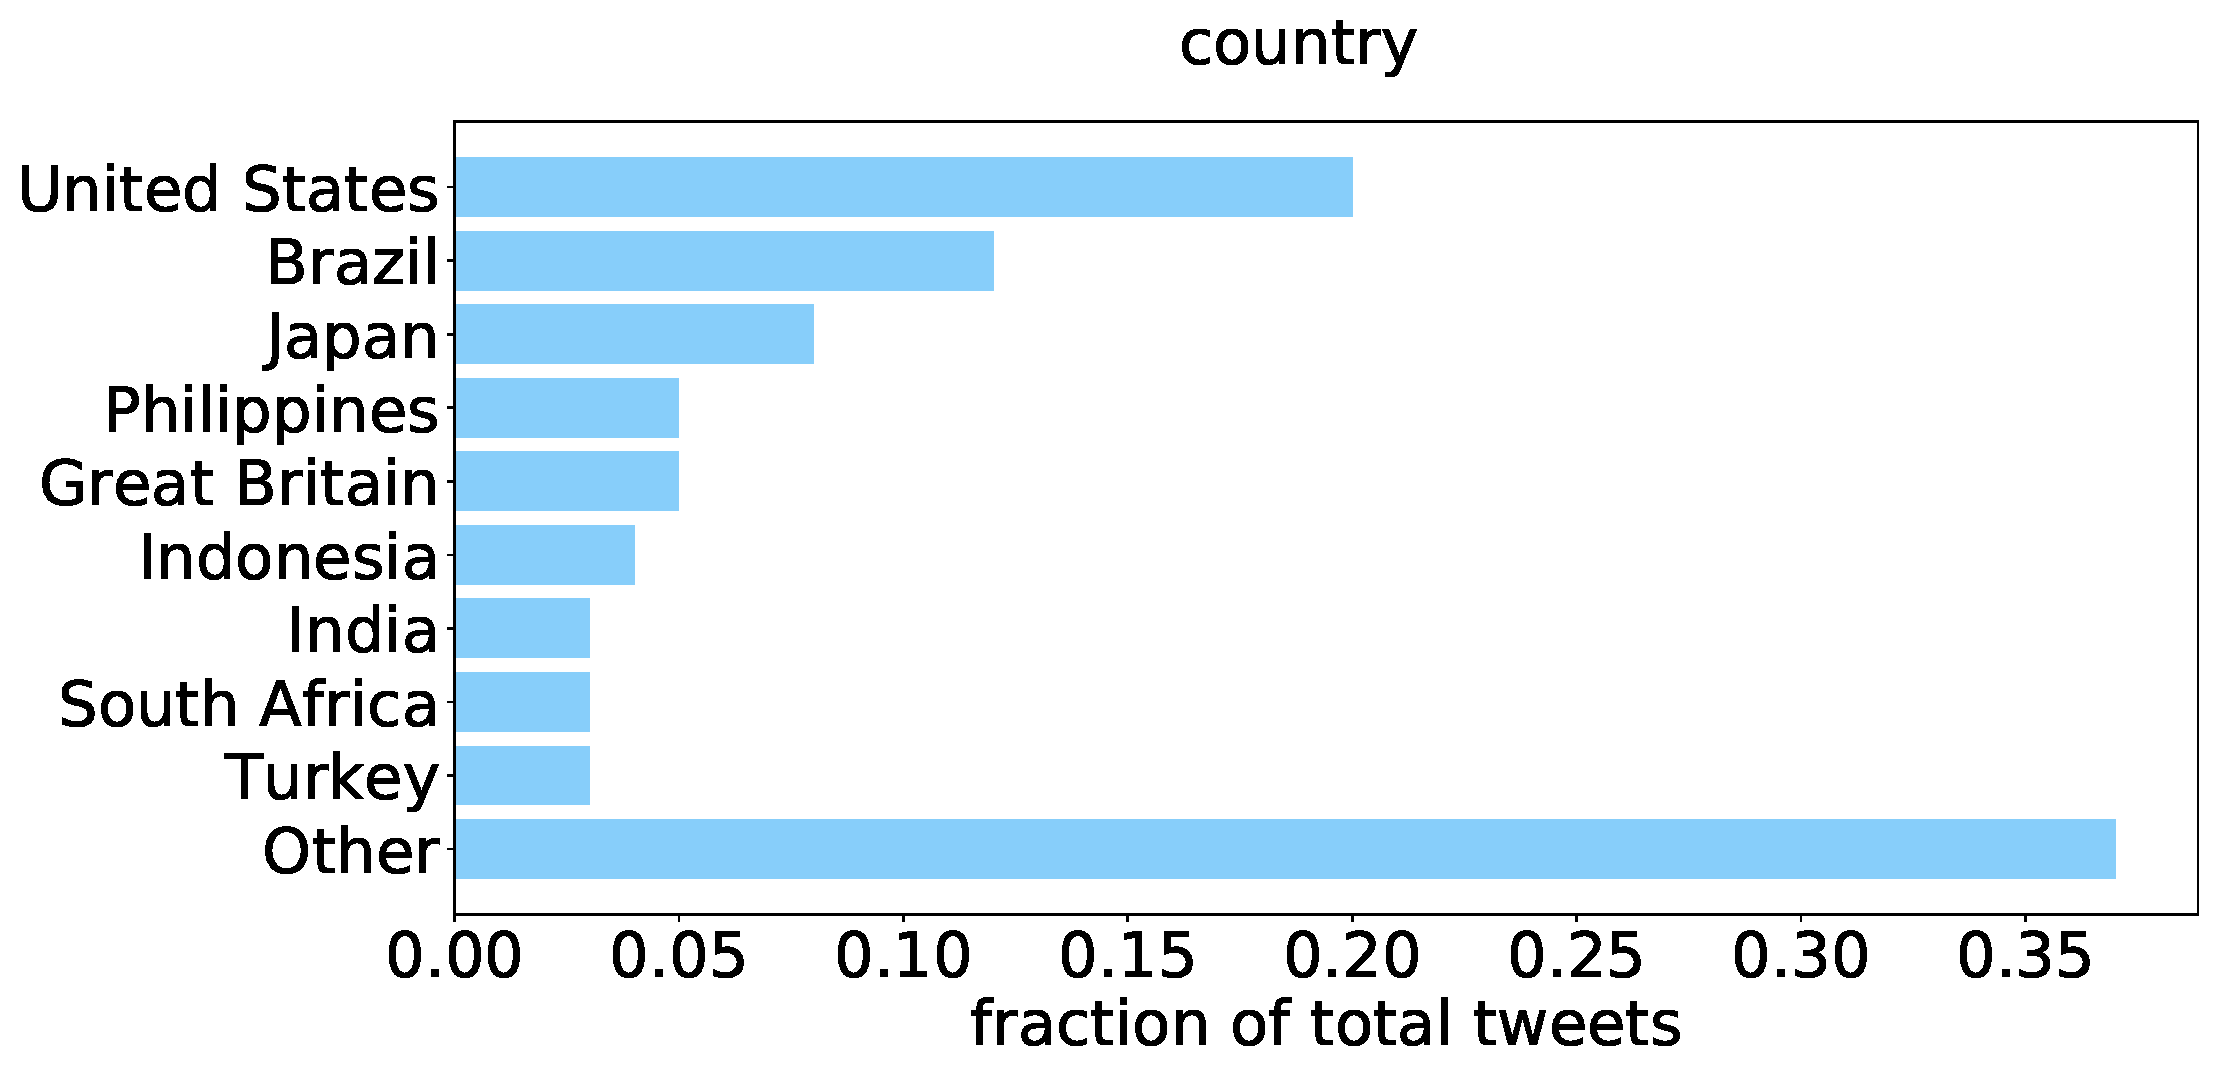
\includegraphics[scale=0.21]{images/countries_fixed.eps}}}%
    \label{adsad}
    \subfloat{{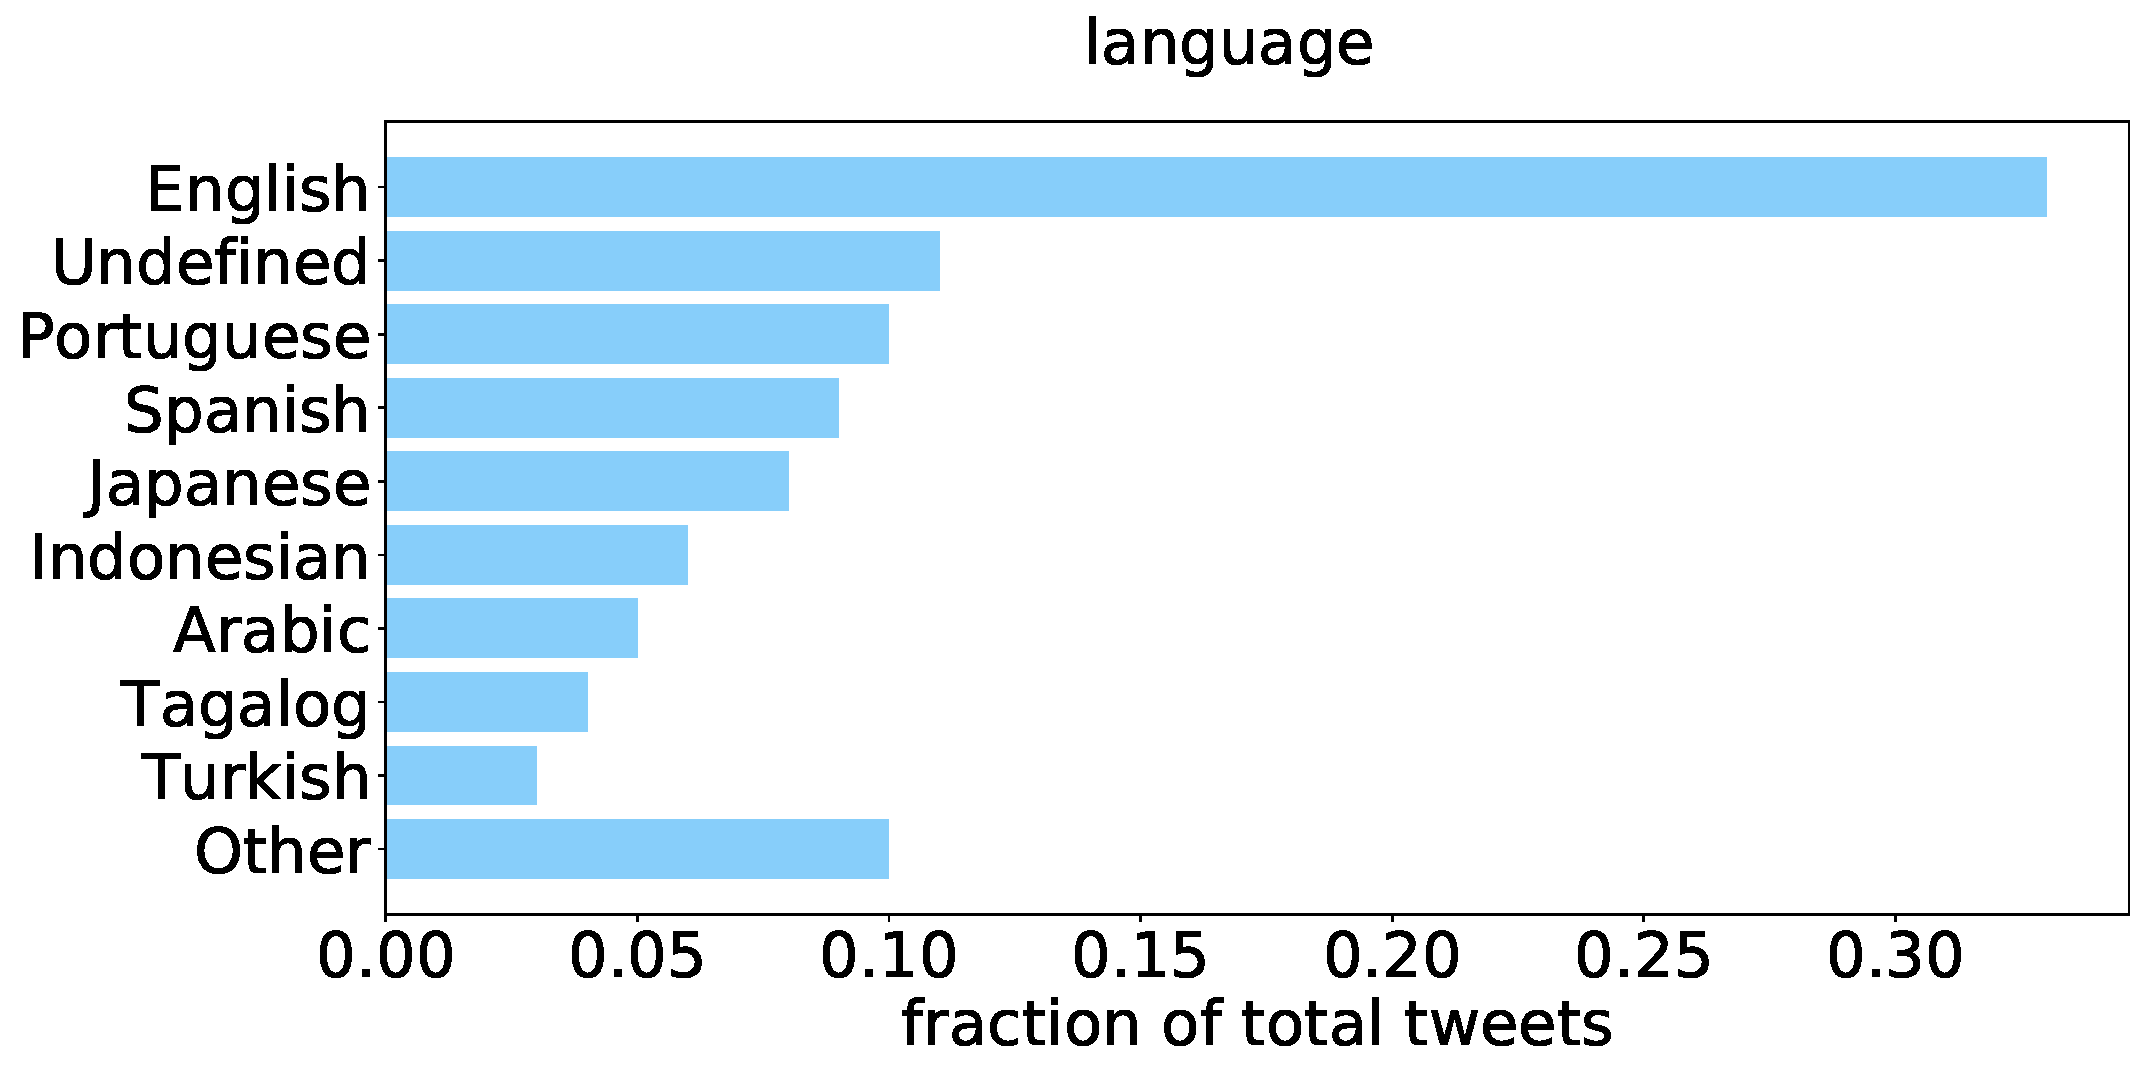
\includegraphics[scale =0.21]{images/languages_fixed.eps} }}%
    \caption{ 
        Stats on the most common countries of origin (\emph{left}) and languages (\emph{right}) for tweets in the $\emoticon$ dataset.
        Languages are determined using Twitter's API, which has official support for 66 languages.
        It is known, however, that more than 100 language are actively used on Twitter \citep{hong2011language},
        and our $\bertmoji$ model supports all of these languages.
        All prior work on emoji prediction has focused on only 1 or 2 languages.
        \fixme{
            The y-axis labels of countries/languages should be horizontal text at the top like a title.
            Generally, we sort from top to bottom rather than bottom to top, so it would be better to flip the order of the y-axis.
            USA would be better as United States since you spell out all the other countries.
        }
    }%
    \label{fig:stats:countrylang}%
\end{figure}

%The $\emoticon$ dataset is specially designed for training the $\bertmoji$ model on tweets related to coronavirus.
The $\emoticon$ dataset is designed for training a classifier that takes as input a tweet and outputs an emoticon that represents the emotion of the tweet.
To generate the dataset, 
we collected all geolocated%
\footnote{
Twitter users can adjust their privacy settings to include different amounts of geolocation metadata.
In particular, they can include the exact GPS coordinate that a tweet was sent from,
an approximate location (for example, the city that the tweet was sent from),
or no location information at all.
We say that a tweet is \defn{geolocated} if any of this metadata is included about the tweet.
Approximately 1\% of all tweets are geolocated.
} 
tweets sent over the six month period between January and June, 2020.
Approximately 400 million tweets meet this criteria.
Then we filtered these tweets so that only tweets containing one of our 80 target emoticons were included,
and any retweets were removed.
In total, the $\emoticon$ dataset contains 64.2 million tweets sent by 4.2 million users.
The tweets are written in 66 different languages and were sent from 246 different countries.
Figure \ref{fig:stats:countrylang} shows the total number of tweets per language,
and Figure \ref{fig:stats:emoticon} shows the frequency of each emoticon in the dataset.

We preprocess each tweet by replacing all user mentions with a special token \texttt{<mention>} and all URLs with a special token \texttt{<url>} and deleting all emojis.
We decided to keep all hashtags because hashtags can contain potentially valuable emotional content useful for emoticon prediction.
Finally, we delete all emoticons from the tweet,
and use the emoticons as the tweet's classification label.
Most tweets have only a single emoticon label, but some tweets have multiple emoticons.
This is a problem because standard multi-class classification techniques require only a single label per data point.
We address the issue by following the procedure established by \citep{felbo2017using}.
If a tweet has multiple emoticons,
then we duplicate it in the training data once for each emoticon,
with each instance being labeled by a single one of the emoticons.
%where for each unique emoji in a tweet, we have a separate tweet with that emoji as a label. 
%For tweets containing repetitions of the same emoji; we only save one instance of it.
%Finally, each tweet is labelled with the emojis that were deleted from the tweet.

\begin{figure}
    \centering
    %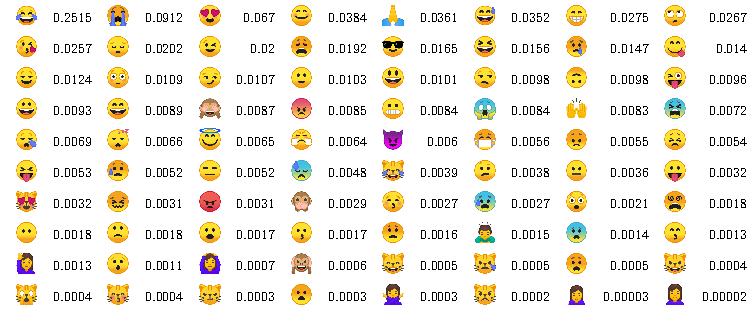
\includegraphics[scale = 1.2]{images/emojitable.pdf}
    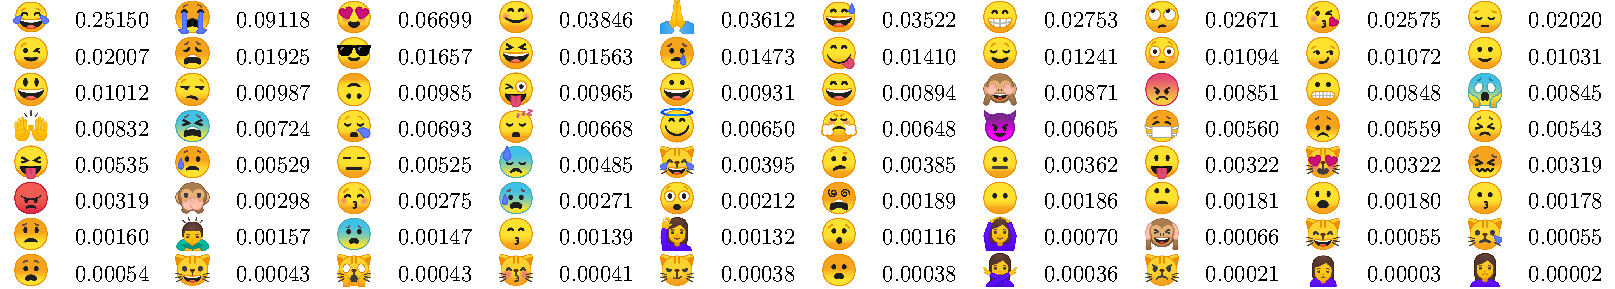
\includegraphics[width = \textwidth,height=1.3in]{images/emoji_table_fix.pdf}
    \caption{
        The 80 target emoticons we are trying to predict,
        and their fraction of all emoticons in the $\emoticon$ dataset.
        The distribution follows a power law.
        %The emoji distribution of the $\emoticon$ dataset.
        %\fixme{All numbers must have either 4 or 5 decimals.  For example 0.02 should be 0.0200}
        %\fixme{The figure needs to take up max 2 inches vertically, but ideally it would be more like 1.5}
    } 
    \label{fig:stats:emoticon}
\end{figure}

We carefully split the $\emoticon$ dataset into training, validation, and test sets ensuring that no user is present in more than one set in order to prevent data leakage.
In particular we assign 80\% of users to the training set, 10\% to the validation set, and 10\% to the test set.
The tweets contained in each set are then the tweets sent by each of the users in the set.

%%%%%%%%%%%%%%%%%%%%%%%%%%%%%%%%%%%%%%%%

\subsection{Training Protocol}

Our $\bertmoji$ model is the multilingual BERT model \citep{devlin2018bert} fine-tuned on the $\emoticon$ dataset.
The multilingual BERT model is a popular model for fine-tuning because it achieves state-of-the-art performance on a wide variety of natural language tasks.
It was trained on data from 102 distinct languages,
and the language of each training sample need not be known for either training or inference.
Followup research has shown that the multilingual BERT model has language-independent internal representations that allow it to encode information from languages it has not seen during training time \citep{pires2019multilingual,wu2019emerging}.
\citet{feng2020language} recently released a more advanced version of the multilingual BERT model that achieves better performance on standard NLP tasks and uses 109 training languages.
We would expect better performance on our emoticon-prediction task using this more advanced multilingual BERT model,
but we did not use this model because all of our experiments were completed before this model was publicly released.

We followed a two step fine-tuning procedure.
First, we trained only the last layer of the model,
generating a model we call $\bertmojill$.
Then, we trained all parameters to generate the $\bertmoji$ model,
warm starting from $\bertmojill$.
We used the validation set to select optimal hyperparameters for both models.
$\bertmojill$ was trained using Adam \citep{kingma2014adam} with a learning rate of $10^{-4}$,
and $\bertmoji$ was trained using Adam with a learning rate of $10^{-5}$.
Both models used a batch size of 64.
A single epoch on the $\emoticon$ dataset took approximately 6 days to run on one NVidia GeForce RTX 2080 GPU.
We trained both models on a single epoch, but found that the model converged before the epoch was finished.
%
%We fine-tuned this pre-trained model to generate two models. 
%The first one only trained the last layer of the model, while the second one trained all the layers.
%We followed the Train-Validation-Test split procedure, where 1 epoch took approximately 6 days to run on one Nvidia GeForce RTX 2080 graphics card.
%The hyper-parameters with which we achieved the highest accuracies are the following. 
%When training the last layer of the model we used: a learning-rate of 1e-04, Adam optimizer and gradient clipping. 
%While training all the layers of the model we had: a learning-rate of 1e-05, Adam optimizer and gradient clipping. 
%Both models were warm-started from previous runs and the batch size used was 64.

%BERT is a new language representation model, which is aimed in pretraining deep bidirectional representations from unlabeled text by jointly conditioning on both left and right context in all layers.
%Therefore, the pre-trained model can be easily fine-tuned by adding another output layer.
%One of the reasons why we picked BERT is due to its performance on the General Language Understanding Evaluation (GLUE) \cite{} benchmark.
%It is comprised of nine language understanding tasks, assembled from a diverse dataset which includes insight into model performance with respect to a wide range of linguistic phenomena.
%At the time of writing, BERT and its variations hold a number of top achieving scores in the GLUE leader-board \ref{leaderboard}.   

\begin{table}
    \centering
    %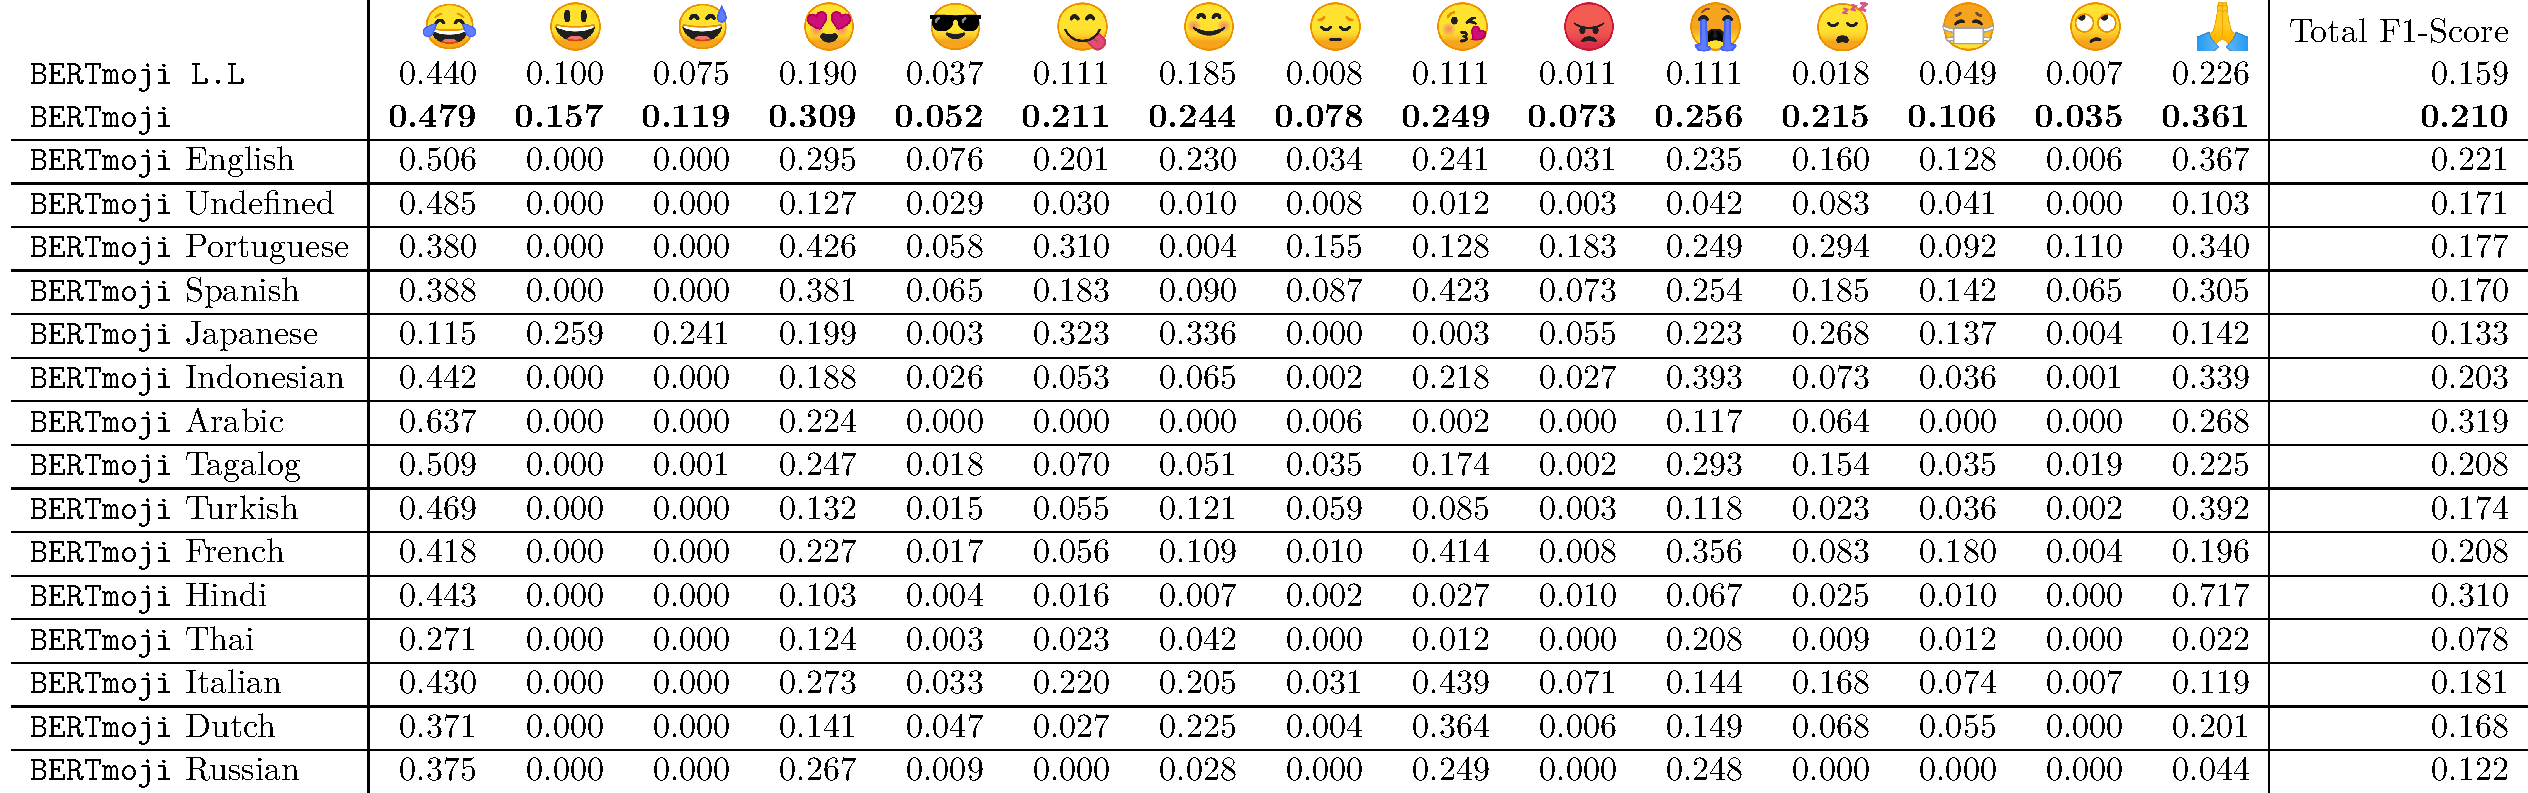
\includegraphics[width=\textwidth]{images/f1_score_table_fix.pdf}
    \resizebox{\textwidth}{!}{
    {\small
\begin{tabular}{lccccccccccccr} 
    %\toprule
%\cmidrule(lr){1}\cmidrule(lr){2-15}\cmidrule(lr){16}
    %\hline
    %\cline{2-15}
    %& \multicolumn{12}{c}{Class-specific F1 scores} & Macro-F1 \\
    %\\

    & \normalsize\emoji{1f602} 
    %& \normalsize\emoji{1f603} 
    %& \normalsize\emoji{1f605} 
    & \normalsize\emoji{1f60d} 
    %& \normalsize\emoji{1f60f} 
    & \normalsize\emoji{1f60b} 
    & \normalsize\emoji{1f60a} 
    & \normalsize\emoji{1f614} 
    & \normalsize\emoji{1f618} 
    & \normalsize\emoji{1f620} 
    & \normalsize\emoji{1f62d} 
    & \normalsize\emoji{1f634} 
    & \normalsize\emoji{1f637} 
    & \normalsize\emoji{1f644} 
    & \normalsize\emoji{1f64f} 
    & Macro-F1
    \\
    \midrule

    \!\!\!\!Model \rule[-0.5em]{0pt}{1em}\\
$\bertmojill$ & 0.440 & 0.190 & 0.111 & 0.185 & 0.008 & 0.111 & 0.011 & 0.111 & 0.018 & 0.049 & 0.007 & 0.226 & 0.159  \\ 

$\bertmoji$ &\textbf{0.479} & \textbf{0.309} & \textbf{0.211} & \textbf{0.244} & \textbf{0.078} & \textbf{0.249} & \textbf{0.073} & \textbf{0.256} & \textbf{0.215} & \textbf{0.106} & \textbf{0.035} & \textbf{0.361} &  \textbf{0.210}  \\ 
    \midrule
    \!\!\!\!Language \rule[-0.5em]{0pt}{1em}\\

Arabic & 0.637 & 0.224 & 0.000 & 0.000 & 0.006 & 0.002 & 0.000 & 0.117 & 0.064 & 0.000 &  0.000 & 0.268 & 0.319 \\ 
Dutch & 0.371 & 0.141 & 0.027 & 0.225 & 0.004 & 0.364 & 0.006 & 0.149 & 0.068 & 0.055 & 0.000 & 0.201 & 0.168 \\ 
English & 0.506 & 0.295 & 0.201 & 0.230 & 0.034 & 0.241 & 0.031 & 0.235 & 0.160 & 0.128 & 0.006 & 0.367 & 0.221  \\  
French & 0.418 & 0.227 & 0.056 & 0.109 & 0.010 & 0.414 & 0.008 & 0.356 & 0.083 & 0.180 & 0.004 & 0.196 & 0.208 \\ 
Hindi & 0.443 & 0.103 & 0.016 & 0.007 & 0.002 & 0.027 & 0.010 & 0.067 & 0.025 & 0.010 & 0.000 & 0.717 & 0.310 \\ 
Indonesian & 0.442 & 0.188 & 0.053 & 0.065 & 0.002 & 0.218 & 0.027 & 0.393 & 0.073 & 0.036 & 0.001 & 0.339 & 0.203 \\ 
Italian & 0.430 & 0.273 & 0.220 & 0.205 & 0.031 & 0.439 & 0.071 & 0.144 & 0.168 & 0.074 & 0.007 & 0.119 & 0.181  \\ 
Japanese & 0.115 & 0.199 & 0.323 & 0.336 & 0.000 & 0.003 & 0.055 & 0.223 & 0.268 & 0.137 & 0.004 & 0.142 & 0.133  \\ 
Portuguese & 0.380 & 0.426 & 0.310 & 0.004 & 0.155 & 0.128 & 0.183 & 0.249 & 0.294 & 0.092 & 0.110 & 0.340 & 0.177 \\  
Russian & 0.375 & 0.267 & 0.000 & 0.028 & 0.000 & 0.249 & 0.000 & 0.248 & 0.000 & 0.000 & 0.000 & 0.044 & 0.122  \\
Spanish & 0.388 & 0.381 & 0.183 & 0.090 & 0.087 & 0.423 & 0.073 & 0.254 & 0.185 & 0.142 & 0.065 & 0.305 & 0.170 \\ 
Tagalog & 0.509 & 0.247 & 0.070 & 0.051 & 0.035 & 0.174 & 0.002 & 0.293 & 0.154 & 0.035 & 0.019 & 0.225 & 0.208 \\ 
Thai & 0.271 & 0.124 & 0.023 & 0.042 & 0.000 & 0.012 & 0.000 & 0.208 & 0.009 & 0.012 & 0.000 & 0.022 & 0.078 \\ 
Turkish & 0.469 & 0.132 & 0.055 & 0.121 & 0.059 & 0.085 & 0.003 & 0.118 & 0.023 & 0.036 & 0.002 & 0.392 & 0.174 \\ 
\rule{0pt}{1em}($*$) Undefined & 0.485 & 0.127 & 0.030 & 0.010 & 0.008 & 0.012 & 0.003 & 0.042 & 0.083 & 0.041 & 0.000 & 0.103 & 0.171  \\  
\bottomrule
\end{tabular}
}

    }
    \caption{
        (\emph{top}) F1 scores for the $\bertmojill$ and $\bertmoji$ models on 12 selected emojis, and the Macro-F1 incorporating all 80 target emoticons.
        The full $\bertmoji$ model offers significantly better performance across all emoji categories.
        (\emph{bottom})
        Performance of the $\bertmoji$ model broken down by language on 15 selected languages.
The Undefined language corresponds to tweets for which the Twitter API was not able to assign a language.
Even for these tweets, which are either written in an unsupported language or do not a significant amount of text within them, the $\bertmoji$ model is able to get performance comparable to many officially supported languages.
        \fixme{Why are the emojis sorted in this order?  I recommend sorting them in order of performance on the $\bertmoji$ model.}
    }
    \label{table:f1}
\end{table}

%%%%%%%%%%%%%%%%%%%%%%%%%%%%%%%%%%%%%%%%

\subsection{Model Evaluation}

The $\bertmojill$ model achieves a Macro-F1 score of 0.159 on the test set and the $\bertmoji$ model achieves a Macro-F1 score of 0.210. Comparatively, top ranked participants of the SemEval 2018 Task 2: Multilingual Emoji Prediction \citep{barbieri2018semeval}, \citep{coltekin-rama-2018-tubingen} achieved F1-scores of 0.3599 in English and 0.2236 in Spanish.
%Afterwards, we performed the classification on the top-15, F1-score achieving emojis. 
%Those emojis comprised about 70 percent of the dataset.
%The results were the F1-scores of 24.07\% and 31.77\% accordingly.
Table \ref{table:f1} shows a performance breakdown by emoji and by language.
Prediction performance on each language varies dramatically because each language uses emojis with different frequencies.
Arabic language tweets, for example, use the ``crying tears of joy'' emoticon (\emoji{1f602}) frequently,
but rarely use the ``smiling face with heart eyes'' emoticon (\emoji{1f60d}).
The model has therefore learned to favor predictions of this emoticon whenever these predictions are present in the tweet.
As Figure \ref{fig:prediction_top10_langs} demonstrates, this causes the same text translated into different languages to receive different emoji labels.
We believe that this is a strength of our model,
as different cultures use emojis differently,
and our model is able to capture this fact.
For some applications, however, it may be more useful to make emoji predictions in a language-agnostic way.
Because the $\bertmojill$ model only trains the last layer of the multilingual BERT model,
it receives no information about the input language,
and provides more language-agnostic emoji predictions. In other words, the model does not take into account the context, idioms or the argot of the language and just uses the core-semantic meaning of the text to generate a emojis.
This language-agnostic approach, however, results in  lower F1 scores since the model does not adapt to those language patterns.

%%%%%%%%%%%%%%%%%%%%%%%%%%%%%%%%%%%%%%%%%%%%%%%%%%%%%%%%%%%%%%%%%%%%%%%%%%%%%%%%

\section{Coronavirus Case Study}
\label{sec:casestudy}

We now apply the $\bertmoji$ model to understand the emotional response of Twitter users to news about the coronavirus.
We first introduce our $\corona$ dataset,
then we present an analysis of this dataset.

\subsection{The $\corona$ Dataset}

\begin{figure}
    \footnotesize
    \emph{%
    bacteria,
    cdc,
    china,
    corona,
    coronavirus,
    cough,
    covid,
    covid-19,
    covid19,
    disease,
    doctor,
    epidemic,
    fever,
    flatten the curve,
    flu,
    lockdown,
    n95,
    ncov,
    nurse,
    outbreak,
    pandemic,
    sars-cov-2,
    sick,
    sinophobia,
    social distancing,
    trump,
    vaccine,
    virus,
    wuhan
}
    \caption{
        The 29 English-language search terms we used to select tweets.
        These terms were translated using Bing Translate into 72 other languages as part of our multilingual tweet filtering process.
    }
    \label{fig:terms}
\end{figure}

The goal of the $\corona$ dataset is to include any geolocated tweet that references COVID-19 in any language.
%We generate the dataset by following a similar procedure as for generating the $\emoticon$ dataset.
%We use dataset is generated by filtering the dataset of 400 million geolocated tweets sent between January and June 2020 that we used to generate the $\emoticon$ dataset.
There is currently no standard procedure for generating multilingual datasets of tweets about a topic,
so we used the following four step procedure:
\begin{enumerate*}[label=(\arabic*)]
\item
    We generated a list of 29 English-language search terms related to the coronavirus,
    as shown in Figure \ref{fig:terms}.
    The choice of terms was inspired by the terms used in a dataset generated by \citet{chen2020tracking},
    but we also removed Twitterisms like ``kungflu'' which would not translate well into non-English languages.
        (We discuss in detail the full differences between our dataset and the dataset of \citet{chen2020tracking} below.)
    Our search terms include generic words like ``china'' and ``trump'' that are not necessarily about the coronavirus,
    but given the time period we searched over,
    many tweets including these terms will be about the coronavirus.
\item
    We then used Bing's translation API to translate each of these terms into the 72 languages supported by Bing translate.
\item
We used Python's $\spacy$ library \citep{spacy2} to tokenize and lemmatize each of the 400 million geolocated tweets sent between January and June 2020.
This is the same time period that we examined for the $\emoticon$ dataset,
and so we hope that the $\bertmoji$ model trained on the $\emoticon$ dataset will transfer well to this $\corona$ dataset.
$\spacy$ supports tokenization in 58 different languages,
and for each tweet we used the appropriate $\spacy$ module for the language specified in the tweet's metadata.
    For languages not directly supported by $\spacy$,
    we tokenized on whitespace.
\item
Finally, the $\corona$ dataset is constructed as the set of all tweets whose lemmatized text contains any of the search terms from the tweet's language or English.
We include both languages in this filtering step because it is common for non-English tweets to use English words like ``coronavirus'' when referencing the virus.
\end{enumerate*}
Figure \ref{fig:lang} shows the full list of 54 languages that are supported by all 3 services.
The $\corona$ dataset contains tweets in an unknown number of other languages,
and the filtering procedure for these unsupported languages used language-agnostic steps,
which likely results in less recall.
In total, 16.2 million tweets meet the criteria to be included in the $\corona$ dataset.

\begin{figure}
    \small
    \emph{%
    Afrikaans,
    %Albanian,
    Arabic,
    Armenian,
    %Basque,
    %Bengali,
    Bulgarian,
    Catalan,
    Chinese,
    Croatian,
    Czech,
    Danish,
    Dutch,
    English,
    Estonian,
    Finnish,
    French,
    German,
    Greek,
    Gujarati,
    Hebrew,
    Hindi,
    Hungarian,
    Icelandic,
    Indonesian,
    Irish,
    Italian,
    Japanese,
    Kannada,
    Korean,
    Latvian,
    %Ligurian,
    Lithuanian,
    %Luxembourgish,
    Malayalam,
    Marathi,
    Norwegian Bokmål,
    Persian,
    Polish,
    Portuguese,
    Romanian,
    Russian,
    Serbian,
    Sinhala,
    Slovak,
    Slovenian,
    Spanish,
    Swedish,
    Tagalog,
    Tamil,
    Tatar,
    Telugu,
    Thai,
    Turkish,
    Ukrainian,
    Urdu,
    Vietnamese
    %Yoruba
    }
    \caption{
        The full list of 54 languages supported by all 3 tools in our processing pipeline (Bing translate, Spacy, and the Twitter API).
        Tweets in other languages are also included in our $\corona$ dataset,
        but the filtering step is less accurate for these unsupported languages.
    }
    \label{fig:lang}
\end{figure}

\begin{figure}
    \centering
    \includegraphics[height=0.6in,width =\textwidth]{images/truevspred_fix.pdf}
    \caption{
        (\emph{top}) The distribution of emotions in the subset of $\corona$ that contain emojis.
        (\emph{bottom}) The distribution of emotions in the subset of $\corona$ that did not contain emojis, and that we used $\bertmoji$ to assign predictions for.
        %The true stacked bar presents the actual Plutchik wheel's mapped responses from the $\corona$ dataset while the predicted stacked bar graph presents the predicted emoji responses mapped to the Plutchik wheel following Figure  \ref{fig:Mapped_emojis} 
        \fixme{the fonts are too small}
        \fixme{the labels should be in the same alphabetical order as Figure 2}
    }
    \label{fig:actual_vs_pred}
\end{figure}

The other significant dataset of coronavirus related tweets was introduced by \citet{chen2020tracking}.
There are two main differences between our dataset and theirs.
First, we only include geolocated tweets,
whereas they include non-geolocated tweets as well.
This results in their dataset being about fifteen times larger than ours,
with about 250 million tweets over the same time period.
Because their data is not geolocated, however, it is not suitable for understanding how different countries have reacted emotionally to COVID-19.
The second difference is that our dataset uses a more advanced language-aware filtering method.
They only search for tweets that contain English keywords.
Most languages, however, have few words in common with English,
and non-Latin based languages frequently do not even use the word ``coronavirus'' to describe the virus.
Chinese tweets, for example, commonly refer to COVID-19 with the string
\begin{CJK}{UTF8}{gbsn}
病毒
\end{CJK},
and Chinese-language tweets containing this string will get included in our dataset but not in their dataset.
As a result of this more advanced processing, the fraction of non-English tweets is much larger in our dataset than theirs (48\% versus 38\%).
Capturing as many non-English tweets as possible about COVID-19 is important for ensuring that our analysis is not unfairly skewed towards English-speaking countries.
%Again, this improves our multicultural analysis in Section \ref{sec:}.

%Importantly, duplicate tweets are included in the $\corona$ dataset,
%but they are not included in the $\emoticon$ dataset.
%This is because of the purpose of the $\emoticon$ dataset. 
%We aimed to apply our $\bertmoji$ to this dataset,
%which is something with free user input where our training data is not fully representative of the eventual data our model will be applied to.
%Therefore this limits our abilities to make assumptions and could possibly inflate our sense of model efficacy.
%On the other hand when dealing with the $\corona$ dataset,
%duplicate inputs result in some distribution on our outputs.
%Since we want to map out the public's emotional response to the coronavirus, it is important 
%for those distributions to be maintained.

%%%%%%%%%%%%%%%%%%%%%%%%%%%%%%%%%%%%%%%%

\subsection{Results}

\begin{figure}
    \centering
    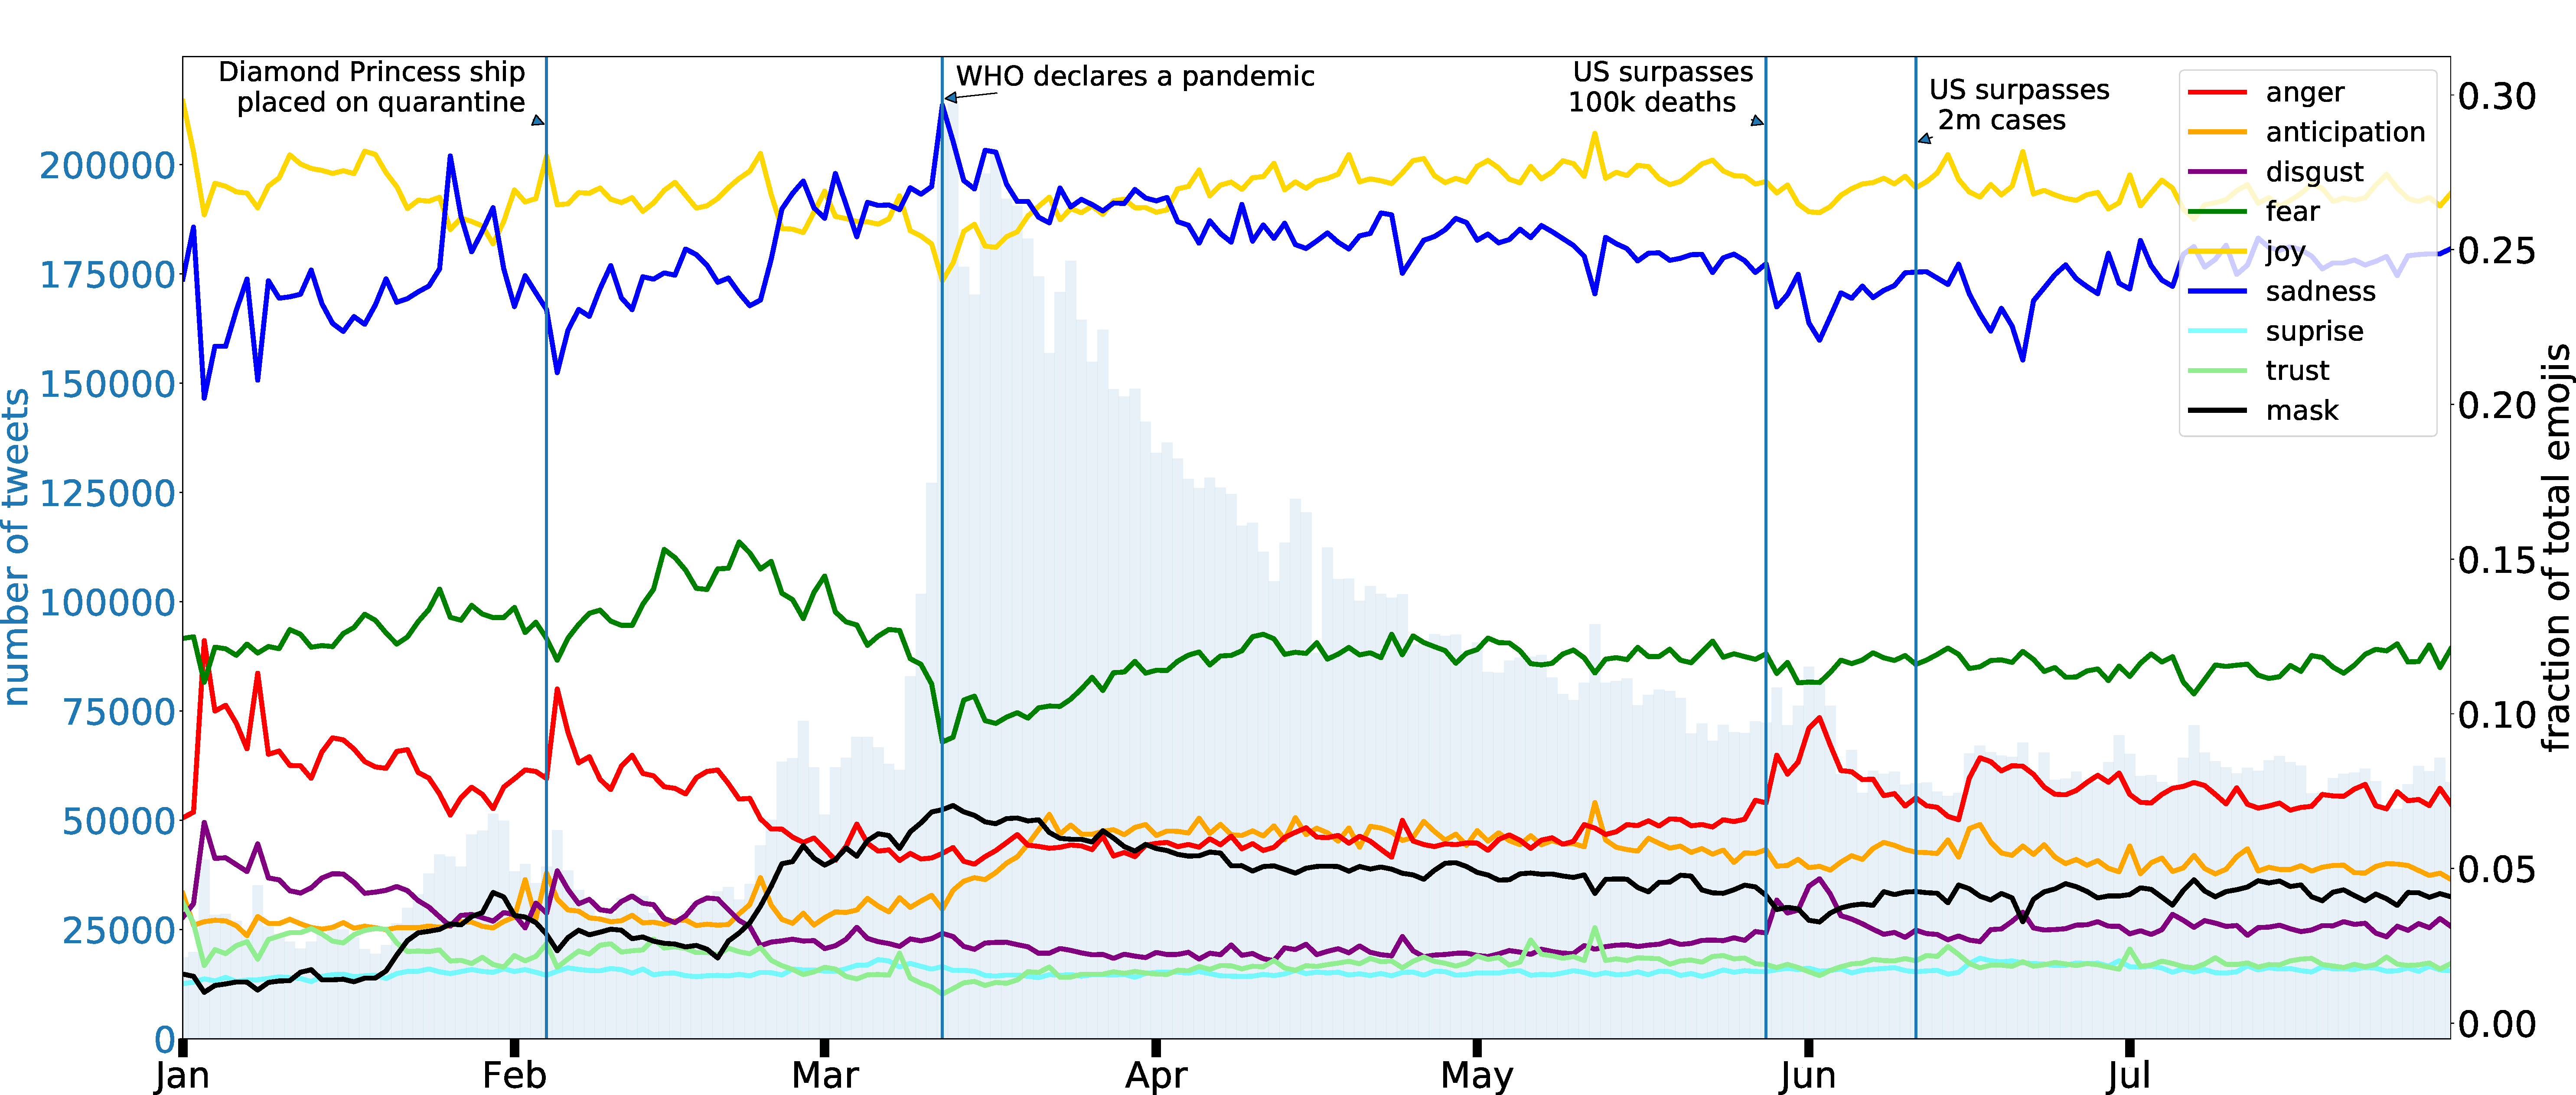
\includegraphics[width=\textwidth,height=2.5in]{images/twitter_sentiment_fixed.pdf}
    \caption{
        The emotional content of tweets in the $\corona$ dataset changes over time and reacts to major news events.
        The shaded bar plot in the background shows the total number of tweets in the $\corona$ dataset sent on a particular day (left y-axis scale),
        and the colored line charts show the fraction of tweets in a particular day that correspond to each emotion on the Plutchik wheel or the mask emoji (right y-axis scale).
        We can see clear emotional reactions to the news events labelled with vertical lines.
        %For example, when WHO declared a pandemic on $\XXX$, we can see a peak in the amount of 
        %\fixme{The fonts are way too small.}
        \fixme{The month names should not be rotated}
    }
    \label{fig:tweets_per_day_sent}
\end{figure}

Only 15.11\% percent of tweets in the $\corona$ dataset contain an emoticon.
We used the $\bertmoji$ model to label the remaining tweet in an effort to capture sentiment included in emoji-free tweets such as the BBC tweet mentioned in the Introduction.
Figure \ref{fig:actual_vs_pred} shows the distribution of tweets present in the dataset vs those we predicted.
The anticipation, disgust, joy, surprise, and trust emoticons appear less frequently in the predicted dataset,
and the anger, sadness, and fear emotions appear more often in the predicted set.
We hypothesize that this difference is due to the fact that more-formal Twitter accounts (such as for newspapers or government organizations) are less likely to use emoji in their tweets,
and these formal accounts also tweet about different topics than more informal accounts of ordinary people.

Our main result is shown in Figure \ref{fig:tweets_per_day_sent}.
For each day, we calculate the fraction of tweets that represent each emotion from the Plutchik wheel (see Figure \ref{fig:Mapped_emojis}),
and we can observe a strong correlation between the emotional content of tweets and important COVID-19 news.
For example, on March 11, the World Health Organization (WHO) declared COVID-19 a worldwide pandemic.
At the same time, we can see a large spike in tweets about the coronavirus,
and in particular we see an increase in sadness and a decrease in joy.
Since sadness and joy are at opposite ends of the Plutchik wheel of emotions,
it makes sense that a rise in one would cause a fall in the other.
%Surprisingly, however, we also see a decrease in the fraction of fear related tweets.
%This surprising result demonstrates that we cannot assume how users will react to news events,
%and we must look at raw data.
As another example, on May 28, the United States had its one hundred thousandth death to the coronavirus.
At the same time, we see spikes in anger and disgust.
The following tweet from this time period is a representative example:
\begin{displayquote}
    How do we tolerate 3000 Americans dying everyday from \#COVID19? THREE. THOUSAND. EVERY. DAY.
\end{displayquote}
This tweet was not originally sent with any emoticons,
but our $\bertmoji$ model was able to label it with \emoji{1f620}, \emoji{mask_photo}, \emoji{1f644}, \emoji{1f62d}. In addition, we highlight an increase in the mask emoji usage around mid-January. Interestingly, at that time little information was available about COVID-19 and protecting yourself against it. Finally, in early February some important news-events that circulated in Twitter were the Diamond Princess Ship being placed under quarantine and the death of Dr Li Wenliang, a Chinese doctor who issued a warning about the coronavirus outbreak before it was officially recognized. At that point we notice a spike in anger and disgust.

%Due to the fact that emojis such as crying-face with tears, dominate the $\emoticon$ dataset,
%we allow the model to predict up to 5 unique emojis for one tweet, to promote more diversity among our results.
%This way, the results can be more meaningful. Further research, can include a more balanced $\emoticon$ dataset.
%We collect the 5 predicted emojis, and after mapping them to the correct sentiment category, we calculate their 
%percent out of the total number of emojis predicted for that day. 
%In order to understand the results we collected all the emojis from the tweets in the $\corona$ and mapped them to the categories in Figure \ref{fig:Mapped_emojis}.  

\section{Conclusion}

We introduced the $\bertmoji$ model for multilingual emoji prediction,
and used this model to better understand how Twitter users responded emotionally to news about the coronavirus.
%We believe we've only scratched the surface of this analysis,
In follow up studies, we hope to analyze how different countries and language communities reacted differently to events,
and have designed our $\corona$ dataset and $\bertmoji$ model to facilitate these cross-sectional analyses.
We also hope that the $\bertmoji$ model will prove useful for analyzing the emotions of text in other contexts outside of COVID-19,
and we make the model available in an easy to use Python package to facilitate this process.

%{ \color{blue} \lipsum[1-2] }

%%%%%%%%%%%%%%%%%%%%%%%%%%%%%%%%%%%%%%%%%%%%%%%%%%%%%%%%%%%%%%%%%%%%%%%%%%%%%%%%
%%%%%%%%%%%%%%%%%%%%%%%%%%%%%%%%%%%%%%%%%%%%%%%%%%%%%%%%%%%%%%%%%%%%%%%%%%%%%%%%
%%%%%%%%%%%%%%%%%%%%%%%%%%%%%%%%%%%%%%%%%%%%%%%%%%%%%%%%%%%%%%%%%%%%%%%%%%%%%%%%
%%%%%%%%%%%%%%%%%%%%%%%%%%%%%%%%%%%%%%%%%%%%%%%%%%%%%%%%%%%%%%%%%%%%%%%%%%%%%%%%
%%%%%%%%%%%%%%%%%%%%%%%%%%%%%%%%%%%%%%%%%%%%%%%%%%%%%%%%%%%%%%%%%%%%%%%%%%%%%%%%

%\bibliographystyle{coling}
\bibliographystyle{plainnat}
\bibliography{main}

\end{document}
